\section{System Evaluation And Case Study}
\label{sec:evo}
\par  In the case study, we use two concrete tasks to demonstrate how investors can apply FKAP to the analysis of movie box office.
\par \textbf{Task 1: Movie Inclusion.} It's important for investors to analyze the performance of a movie. Movie performance not only refers to box office income, word of mouth, but also includes the changes in the audience and the change of the influence of the director during the screening process.

\begin{figure}[!htbp]
\centering
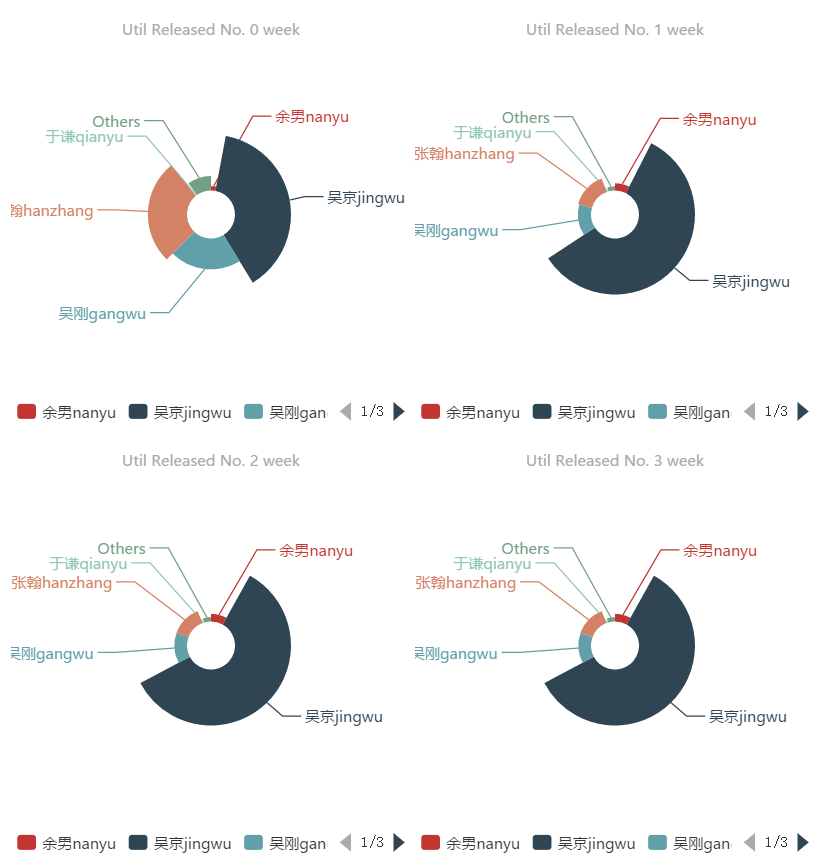
\includegraphics[width=0.8\columnwidth]{case1.png}
\caption{Dynamic Impact of Wolf Warriors II}
\label{fig:case1}
\end{figure}

\par Fig.4 shows dynamic impact of creators in "Wolf Warriors II". Before the movie released (week 0), the attentions people payed to Hans Zhang, Gang Wu and Jason Wu were equal while with the movie's release and the increase in the heat of the film, more and more people went to the movies for the sake of Jason Wu. Meanwhile, the dynamic influence process can reflect a major change in the importance of the movie. We can see that Jason Wu has greatly improved his value through the movie himself. To some extent, Jason Jing has more box office attractiveness, and investing in the actor's next movie is very likely to get high box office gains.

\par \textbf{Task 2: Evaluation of investment quality.} Investors usually need to assess the movie's expected box office and measure the actor's return on investment. Because there is a strong correlation between movie box office and audience feedback, the box office of the first week is less affected by audience feedback, so the first week box office can be regarded as the baseline of box office. The first week box office prediction can measure the expected revenue of the movie, and the actor replacement module can help investors to screen the appropriate actors at the right price at the appropriate box office in the first week.

\par In \system, we give a interface to query expected box-office when combine many factors into an investment. Such as Chinese actor $ YangMi$ and $YifengLi$ and year selector into $2017$ winter, the expected outcome is $184.55$ million. We confirm the result as table \ref{tab:pred} shows. The data indicated that two star co-star relation really play an important role in box-office improvement compared with single star.

\begin{table}[!htb]
  \centering
  \begin{tabular}{c|c|c|c}
  \hline
  Actors & year & schedule & Outcome\\
  \hline
  YangMi + YifengLi& $2017$ & Winter & $184.55$ m  \\
  \hline
  YangMi + YifengLi& $2016$ & May Day & $143.83$ m\\
  \hline
  YifengLi& $2016$ & May Day & $123.60$ m\\
  \hline
  \end{tabular}
  \caption{Estimate first week box-office for future investment}
  \label{tab:pred}
\end{table}

\par \textbf{Task 3: Quantify sentiment and choose suitable actor.} The following part will show the film sentiment analysis. Taking a pretty hot film Kung Fu Yoga in 2017 into consideration, at the first ten days, positive sentiment control the major opinion. While as time goes on, negative sentiment active peak much higher than normal positive sentiment. We can see form figure \ref{fig:case3} that people begin to criticize Jack Chen about this film. Even though at last, the public sentiment turn steady, we still believe Kung Fu Yoga has a tough time.

\begin{figure}[!htbp]
\centering
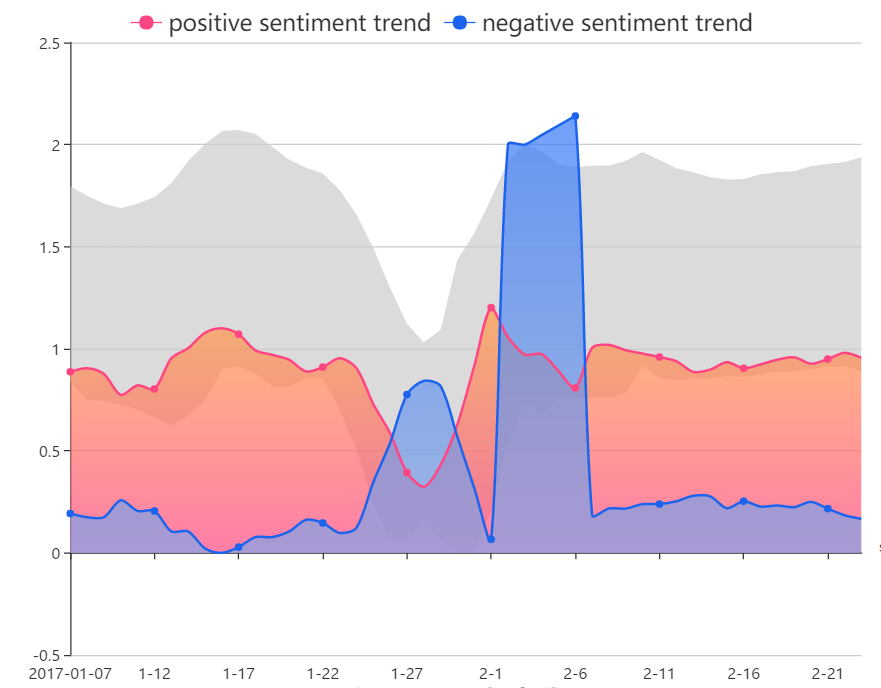
\includegraphics[width=0.8\columnwidth]{case3.png}
\caption{Film trend of Kung Fu Yoga}
\label{fig:case3}
\end{figure}

At last, we want to give a rank list of alternative actors when investors choose major actor. We give rank order form both AMTMA and AMDMA meta-path based method. If we query $JingWu$ (Chinese major actor of  Wolf Warriors II), we get highest score of 4.43 for Chow Yun Fat( Famous Chinese actor) based on his performers' experience especially film types that has been played in. Table \ref{tab:alter} give details.

\begin{table}[!htb]
  \centering
  \begin{tabular}{c|c}
  \hline
  Alternative Actor Name & rank score\\
  \hline
  yun-fatchow & 4.43  \\
  \hline
  qianyuanWang & 4.38\\
  \hline
  qingYe & 4.38\\
  \hline
  tomeroz & 4.36\\
  \hline
  hakonFung & 4.35\\
  \hline
  \end{tabular}
  \caption{Highest 5 recommend alternative actors for JingWu}
  \label{tab:alter}
\end{table}
